        \insertmeeting 
	{Meet 5} 
	{01/14/23} 
	{Rockledge High School}
	{Ritam, Mohana, Jensen, Nathan, Robert, Karissa, Tyler, Samantha}
	{Images/RobotPics/robot.jpg}
	{9:00 - 5:00}
	
\hhscommittee{Hardware}
\noindent\hfil\rule{\textwidth}{.4pt}\hfil
\subsubsection*{Goals}
\begin{itemize}
    \item Meet 5!

\end{itemize} 

\noindent\hfil\rule{\textwidth}{.4pt}\hfil

\subsubsection*{Accomplishments}
Walking into this meeting, we were… not confident to say the least. Our robot had been going under major revisions over the past month to incorporate an intake arm in the back, and a new outtake, a new cart design that would drop off the cones without the usage of a servo. The thing about a change like this is that it’s incredibly risky, and we did not roll snake eyes this time around. Our robot was barely functioning, and while the hardware was enough to technically score cones, there was no time for software to do anything, so the hardware didn’t mean much at the end of the day. The autonomous we were using was all the way back from meet 1, when we were a push bot, which came in handy for scoring the parking points fairly consistently, but isn’t a nice thing to admit. Overall, we weren’t expecting much from today.
For hardware, everything barely worked in our matches. Our intake wasn’t very grippy and the funnel was made to exactly fit the cones, which was a mistake since our funnel wasn’t made properly, so we had to position our robot in a pretty exact spot to pick cones up. Our cart wasn’t much better. Sure, it could score when the pulley didn’t get tied up on something, but the junctions would wobble around a ton when doing so, since they needed a large amount of force to rip the cones off. This was an intentional choice however, since if we didn’t have anything stopping it, the cone would fly off when stopping after moving forward. Either way, even if it worked consistently, it would still be slow. It’s a struggle to rip the cone off the top of the junction, and waiting for the cart to go down to the bottom before moving still wastes time. Going forward, we need to fix up the issues with the intake, and change the outtake design to a traditional servo-based one.
Software went even worse, but not to any fault of their own. Due to our hardware committee taking too long, they were simply dealt a bad hand, and pretty much had to start on the code the day of the competition. And they had a lot to do, with an entire intake to work out. It’s hard to say what went wrong considering their faults laid more on hardware, but going forward, it’s very important they are given the time to program the intake and an autonomous.

Here’s how our matches went:

In our first match, we lost 46-59, contributing 24 points ourselves. A cone got stuck in our cart, so the only points we scored were the parking points in auto and endgame. While we lost, it was close enough to show that despite this being the last meet before League Championships, we could still win some matches with a bit of luck.

In our second match, we lost 69-105. The malfunction this time was the poles nearly getting stuck on our intake, but after shaking it off during Tele-Op, the pulley pulling the cart got stuck and we couldn’t hand off any cones even if we could pick them up with our intake. About the same song and dance, maybe we could get lucky, but not this time.

In our third match we scored 0-27. Our alliance partner didn’t come, and our robot never initialized, and we have no clue why. Maybe the code didn’t download properly, or maybe it was static electricity in the field, as a member of team 7592, Roarbots, pointed out to us. Either way, we just tried to keep a happy face on as we awkwardly stood there during the match.

Our fourth match was our first win of the day, 94-47, with us contributing 30 points. We got lucky with our alliance partner, 16290, ZIP Ties, being able to score enough to pick up our dead weight, but using our preloaded cone, we scored our first cone of the day! It was exhilarating to see things turn up a bit, but it should be noted that, as mentioned before, it caused the pole to wobble a lot, and wasn’t fast enough to effectively cycle, and watching the robot struggle with releasing the cone certainly showed that.

Our fifth match was yet another win, 66-57. With us contributing another 30 points. Not much new to note here, things went similarly to the past match

We got really lucky with our sixth match, scoring 156-52, the high score for the day… until the match that followed. We once again scored 30 points, and outside of our alliance partner, 18172, Uplift Robotics, doing incredibly well, nothing really changed.

At the end of the day, we didn’t do so hot. We scored very few cones, and nothing really improved from the last meet. That is, except our ranking. We risen 1 rank, from 6th to 5th, which, despite everything that happened today, we count as a win. Sure, it’s not our proudest moment, but we didn’t lose hope, and we got a little something for our efforts. For Leagues, we need to finish up the hardware kinks on the intake, create a new cart, and improve our software.

 

\begin{figure}[ht]
\centering
\begin{minipage}[b]{.48\textwidth}
  \centering
  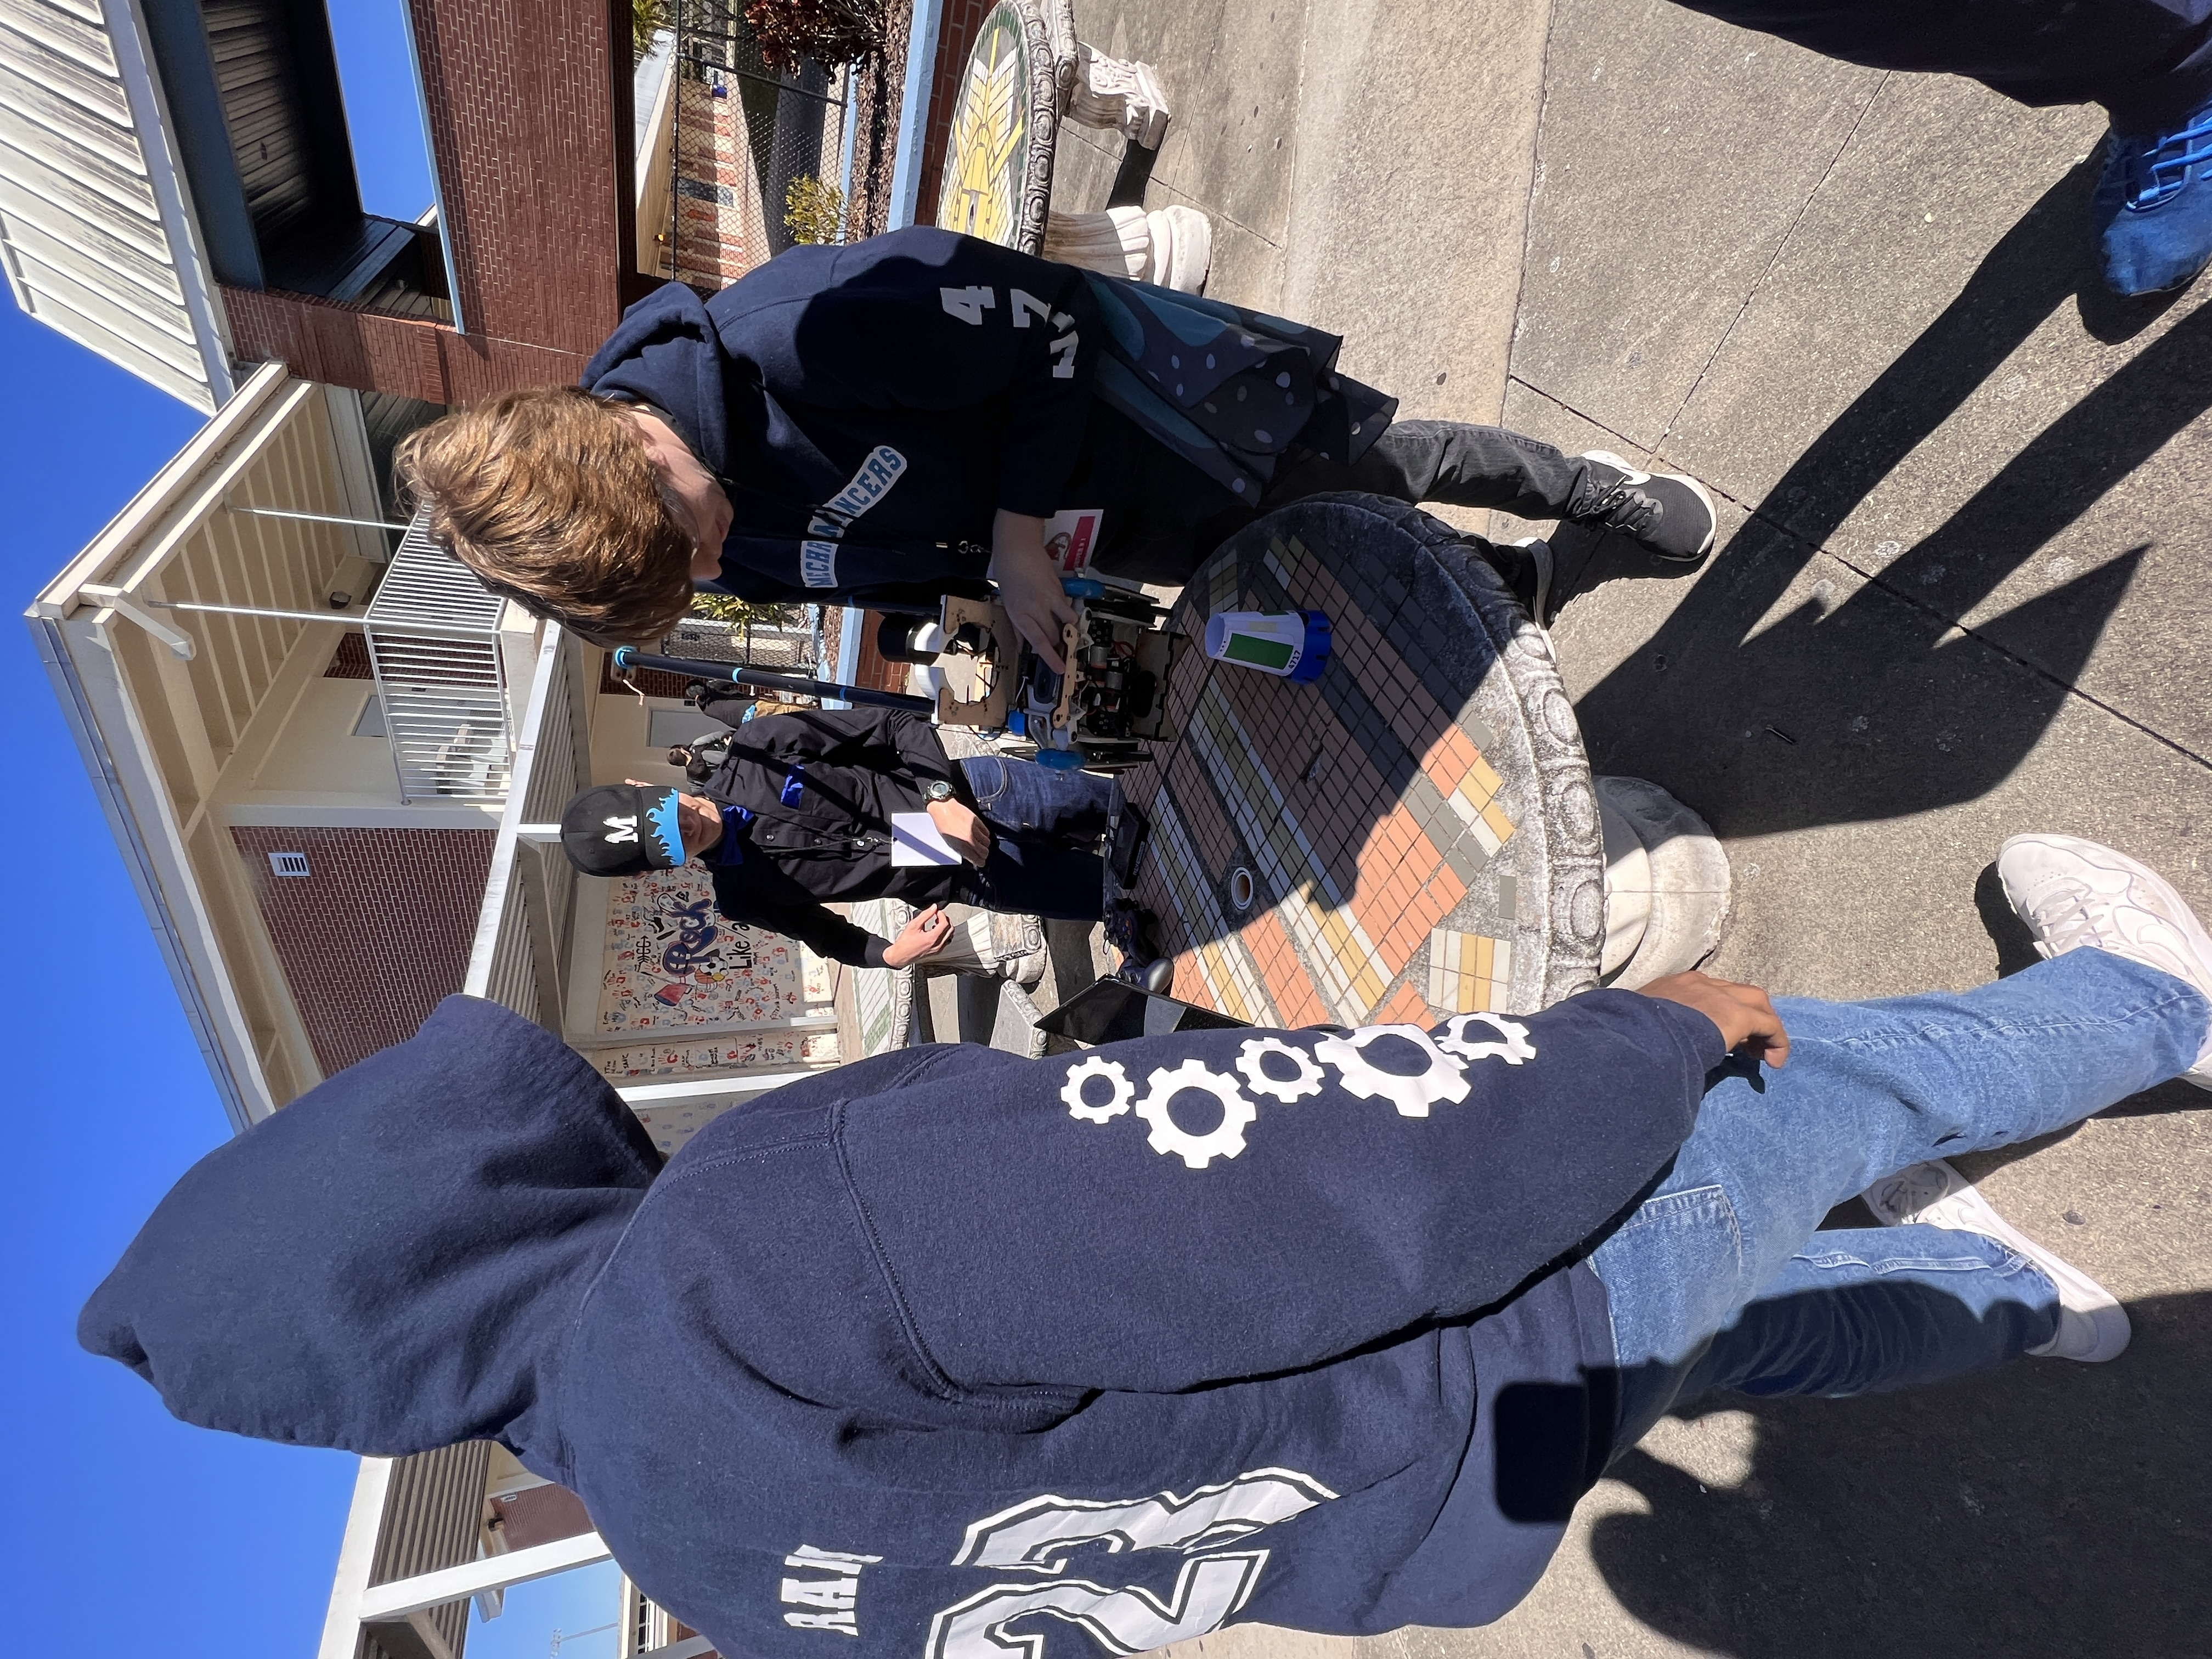
\includegraphics[width=0.95\textwidth]{Meetings/January/01-14-23/01-14-23-Hardware.JPG}
  \caption{Meet 5}
  \label{fig:pic1}
\end{minipage}%
\hfill%
\begin{minipage}[b]{.48\textwidth}
  \centering
  \includegraphics[width=0.95\textwidth]{Meetings/January/01-14-23/01-14-23-Hardware1.JPG}
  \caption{Meet 5}
  \label{fig:pic2}
\end{minipage}
\end{figure}


\whatsnext{
\begin{itemize}
    \item Reflect on our performance from this meet
    \item Review mistakes and sources of failures
    \item Propose new ways to improve what we currently have
\end{itemize} 
}
